\documentclass[12pt]{article}
\usepackage{amsmath}
\usepackage{geometry}
\usepackage{setspace}
\usepackage{graphicx}
\usepackage{hyperref}
\usepackage{float}
\usepackage{svg}
\usepackage{booktabs}


% Margins
\geometry{letterpaper, margin=1in}


% Font
\usepackage{helvet}
\renewcommand{\familydefault}{\sfdefault}
\renewcommand{\normalsize}{\fontsize{11}{13}\selectfont}
\renewcommand{\large}{\fontsize{12}{14}\selectfont}
\normalsize

% Section formatting
\usepackage{titlesec}
\titleformat{\section}
  {\normalfont\bfseries}
  {\thesection.}{1em}{\underline}
\renewcommand{\thesection}{\Alph{section}}

% Subsection formatting
\usepackage{titlesec}
\titleformat{\subsection}
  {\normalfont}
  {\thesubsection}{1em}{\underline}
\renewcommand{\thesection}{\Alph{section}}

% Version
\usepackage{fancyhdr}
\fancypagestyle{plain}{
  \fancyhf{}
  \fancyhead[R]{V1 9/2023}
  \renewcommand{\headrulewidth}{0pt}
}
\pagestyle{plain}

% ReLU^2
\newcommand{\reluTwo}{$\text{ReLU}^2$}


\title{Final Research Report}
\author{Scott Chase Waggener}

\begin{document}

% Page numbers
\fancypagestyle{plain}{
  \fancyhf{}
  \fancyfoot[C]{\thepage}
  \fancyhead[R]{V1 9/2023}
  \renewcommand{\headrulewidth}{0pt}
}
\pagestyle{plain}


\begin{titlepage}
    \centering
    \vspace*{1in}
    \large \textbf{AIM-AHEAD RESEARCH FELLOWSHIP COHORT 2} \\
    \vspace{1\baselineskip}
    \large \textbf{Final Research Report} \\
    \vspace{2\baselineskip}
    \raggedright
    \textbf{Research Project Name: MiT-UB: A Multi-Domain Unbiased Medical Vision Foundation Model} \\[2\baselineskip]
    \large \textbf{Research Fellow Name:} Scott Chase Waggener \\[2\baselineskip]
    \large \textbf{Research Fellow Institution:} University of Texas at Dallas \\[2\baselineskip]
    \large \textbf{AIM-AHEAD Mentor Name:} Jay Patel \\[2\baselineskip]
    \large \textbf{Institutional Mentor Name:} Lakshman Tamil
\end{titlepage}

\newpage
\section{Research Abstract}
\noindent
This work presents MiT-UB, a novel deep learning architecture based on Vision Transformers
(ViTs), tailored for the critical task of breast cancer triage. Leveraging the advanced capabilities
of ViTs, which have shown remarkable success in image analysis, we adapt this technology to
medical imaging with the goal of enhancing early and precise detection of breast cancer.
A thorough set of ablation studies using CIFAR-10 inform the design of MiT-UB, achieving a maximum test accuracy of
$87.5\%$ with supervised fine-tuning and $81.97\%$ with linear probing, while not relying on external data or models.
This optimized design was applied to the medical domain where we propose AViT, an adaptive vision transformer architecture
well suited to high resolution data. Through multiple pre-training stages and a supervised fine-tuning stage we optimize
MiT-UB for breast cancer triage. An enriched test dataset of $4208$ mammograms from $1052$ patients is curated from the EMBED dataset, on which MiT-UB achieves an AUROC of $0.8494$. Subsequent stratified analysis of performance by patient race
suggests unbiased performance, though representation of certain minority subgroups is limited. 


\section{Research Question, Aims, and Goals}
\noindent
% Describe the specific approach you took for your research; specifically outline the research question, aims, goals, objectives, deliverables, and timeline. (250 words or less)

\underline{The project asks the following research questions:}
\begin{itemize}
    \item How accurately can a vision foundation model determine the presence of malignant lesions in a screening mammogram?
    \item Is it possible to reduce bias in computer vision algorithms?
\end{itemize}

\underline{The project has the following aims:}
\begin{itemize}
    \item Aim 1: Develop, test, and validate deep learning models to automatically diagnose breast cancer cases.
    \begin{itemize}
        \item Aim 1.1: Develop a foundation model (MiT-UB) tailored to medical imaging that can generalize to a diverse range of modalities and populations.
        \item Aim 1.2: Architect MiT-UB such that it is a viable foundation model for as many patient populations, imaging modalities, and use cases as possible.
        \item Aim 1.3: Curate a highly diverse training set suitable for pre-training this model.
        \item Aim 1.4: Assess the performance of the model when fine-tuned to detect the presence of malignant lesions in screening mammograms.
    \end{itemize}
    \item Aim 2: Analyze and mitigate bias within MiT-UB.
    \begin{itemize}
        \item Aim 2.1: Apply unsupervised pre-training and supervised fine-tuning to MiT-UB using the diverse dataset curated in Aim 1.3.
        \item Aim 2.2: Quantify the model’s ability to identify the presence of malignant lesions in an unbiased manner.
    \end{itemize}
\end{itemize}

\underline{The project has the following deliverables:}
\begin{itemize}
    \item Technical report on the architecture and training procedure for MiT-UB.
    \item Performance report of MiT-UB for breast cancer triage, including stratified analysis.
\end{itemize}


\section{Study Design and Methodology}
\noindent
% Describe the study design and methods you used in the research project. (500-1000 words)

\subsection{Data}

Initial evaluation and ablations of the M-JEPA architecture were conducted using the CIFAR-10 \cite{krizhevsky2009learning} image dataset. 
CIFAR-10 consists of 60,000 32x32 color images in 10 classes with 6,000 images per class, making it an excellent dataset for prototyping and evaluation of deep learning models.
We follow the train/test partition defined by the creators of the CIFAR-10 dataset, using the training partition for both self-supervised and supervised training. \cite{krizhevsky2009learning}

Two datasets are leveraged to evaluate the M-JEPA architecture in the medical domain. For final performance testing, we leverage the $20\%$ of the EMBED \cite{embed2023} dataset made
available to the AWS Open Data program. 

An independent training set was prepared consisting of 452,952 unique mammograms across 
six data sources spanning five continents, representing 30,906 unique patients. This dataset consists entirely of female patients,
and includes data licensed or purchased by MedCognetics Inc. from 2020 to 2023 from the U.S., U.K., Germany, India, Brazil, and Nigeria. The mean age at examination is $59.17$ years.
Standard mammographic screening exams from an additional 821 female patients were used to evaluate the performance of the M-JEPA architecture. Ground truth for this validation set
was established through biopsy confirmation or two year stability. 
These exams were sourced from U.S. based clinical sites not included in the training set to ensure independence of training and validation data.

Final performance testing and stratified analysis was conducted using EMBED. The data available through the AWS Open Data program is comprised of $72924$ mammography studies from $23256$ patients. Of these, $72922$ studies are  full-field digital mammography (FFDM) exams and $29961$ are synthetic 2D.
There is substantial representation of African American ($N=9561$) and White ($N=8641$) patients, with lower representation for Hispanic ($N=1270$), Asian ($N=1552$), and Native American ($N=62$) patients. The BIRADS breast density distribution roughly follows the distribution of the general U.S. population ($\mathrm{A}=2036$, $\mathrm{B}=9328$, $\mathrm{C}=10128$, $\mathrm{D}=1579$). Most mammograms were captured using Hologic machines ($N=447496$), with minority representation from GE ($N=30590$) and Fujifilm ($N=8247$).

EMBED provides detailed pathology from which a binary malignancy label can be established for each exam. Using the taxonomy
of breast pathology defined in \cite{embed2023}, we consider "Invasive Cancer", "Non-Invasive Cancer", and "Non-Breast Cancer" to be malignant, and all other pathologies to be benign. This yields $995$ malignant studies and $72106$ benign studies.
To curate the final test set we consider only complete screening exams (having both left and right medio-lateral oblique and cranio-caudal views). For patients with one or more studies having a malignant finding, we select the earliest malignant screening exam.
Otherwise, we select the earliest benign study thereby maximizing the window of known stability. 
Finally, to enrich the test set, we include all malignant studies meeting the above criteria along with an equal number of benign studies. 
This yields $526$ malignant and $526$ benign studies in the test set, for a total of $4208$ mammograms.

\subsection{Architecture}

The Vision Transformer (ViT) \cite{dosovitskiy2020vit} is chosen as the base architecture for MiT-UB due to its proven effectiveness in image recognition tasks and viability as a foundation model. From this base architecture we apply several
modifications to improve its performance and facilitate scaling to high resolution inputs. Two variations of MiT-UB are
considered: one that more closely resembles the standard ViT architecture and one that is specifically designed for high resolution inputs. The high resolution backbone is designed to adapt to varying resolutions
and is referred to as the Adaptive Vision Transformer (AViT).

The design of the standard ViT architecture is shown in Figure \ref{fig:vit}. An input image is divided into a grid of non-overlapping patches, each of size $P \times P$. 
Patches are then flattened into a sequence of tokens, which are embedded into a feature space using a linear layer.
Multiple transformer layers are applied to the sequence of tokens, with self attention and MLP layers interleaved. 
The output of the ViT backbone is a sequence of feature vectors, equal in length to the number of patches in the input image.

\begin{figure}[H]
    \centering
    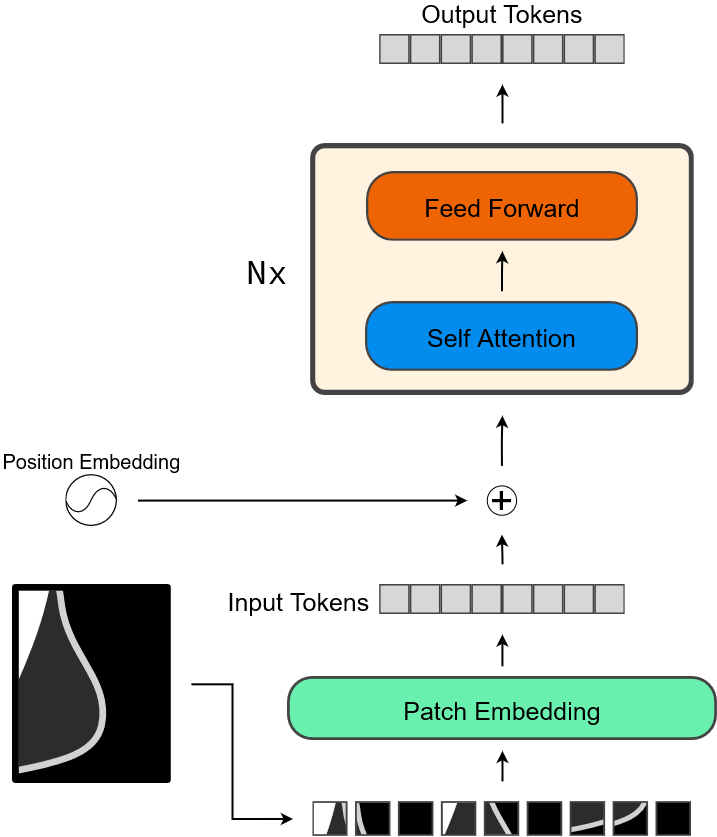
\includegraphics[width=0.6\textwidth]{./figures/vit.png}
    \caption{Standard Vision Transformer (ViT) Architecture}
    \label{fig:vit}
\end{figure}

Since the ViT architecture is permutation invariant, positional information is injected in the form of a positional embedding.
MiT-UB adopts a factorized fractional position encoding to improve the model's ability to generalize to high resolution inputs, which is depicted in Figure \ref{fig:position-encoding}. 
Token positions are normalized to a coordinate in the range $[-1, 1]$ and fed as independent features into a single linear layer. The output is a position embedding which is added to the original token embedding.


\begin{figure}[H]
    \centering
    \includesvg[width=0.6\textwidth]{./figures/pos_enc.svg}
    \caption{Factorized fractional position encoding used by MiT-UB. Token coordinates are normalized to the range $[-1, 1]$ and fed into a single linear layer as independent features to produce a position embedding.
    }
    \label{fig:position-encoding}
\end{figure}


Squared ReLU (\reluTwo) \cite{so2022relu2} is adopted as the default activation function for all MLP layers in the ViT backbone. Biases are omitted from all attention and MLP layers.


Scaling a standard ViT to the resolution of mammograms is prohibitively expensive in terms of memory and compute, due to the quadratic complexity of the self attention operation.
To address this we modify the standard ViT to perform cross-attention between a fixed number of pooled query tokens and the high resolution input tokens. This approach draws inspiration
from architectures like the Perceiver \cite{jaegle2021perceiver}, GPViT \cite{yang2023gpvit}, and ViTAR \cite{fan2024vitar}. First, the high resolution set of tokens are adaptively pooled to a
fixed size using either average or max pooling. These pooled tokens are then processed using a standard ViT self attention backbone. To recover high resolution information a series of
additional transformer layers are added which incorporate a cross-attention operation using the pooled tokens as queries and the high-resolution input tokens as keys and values. 
This approach makes AViT non-quadratic in computational complexity with respect to the input sequence length, making it suitable for the high resolution input data found in medical images.
The design of AViT is shown in Figure \ref{fig:avit}.

\begin{figure}[H]
    \centering
    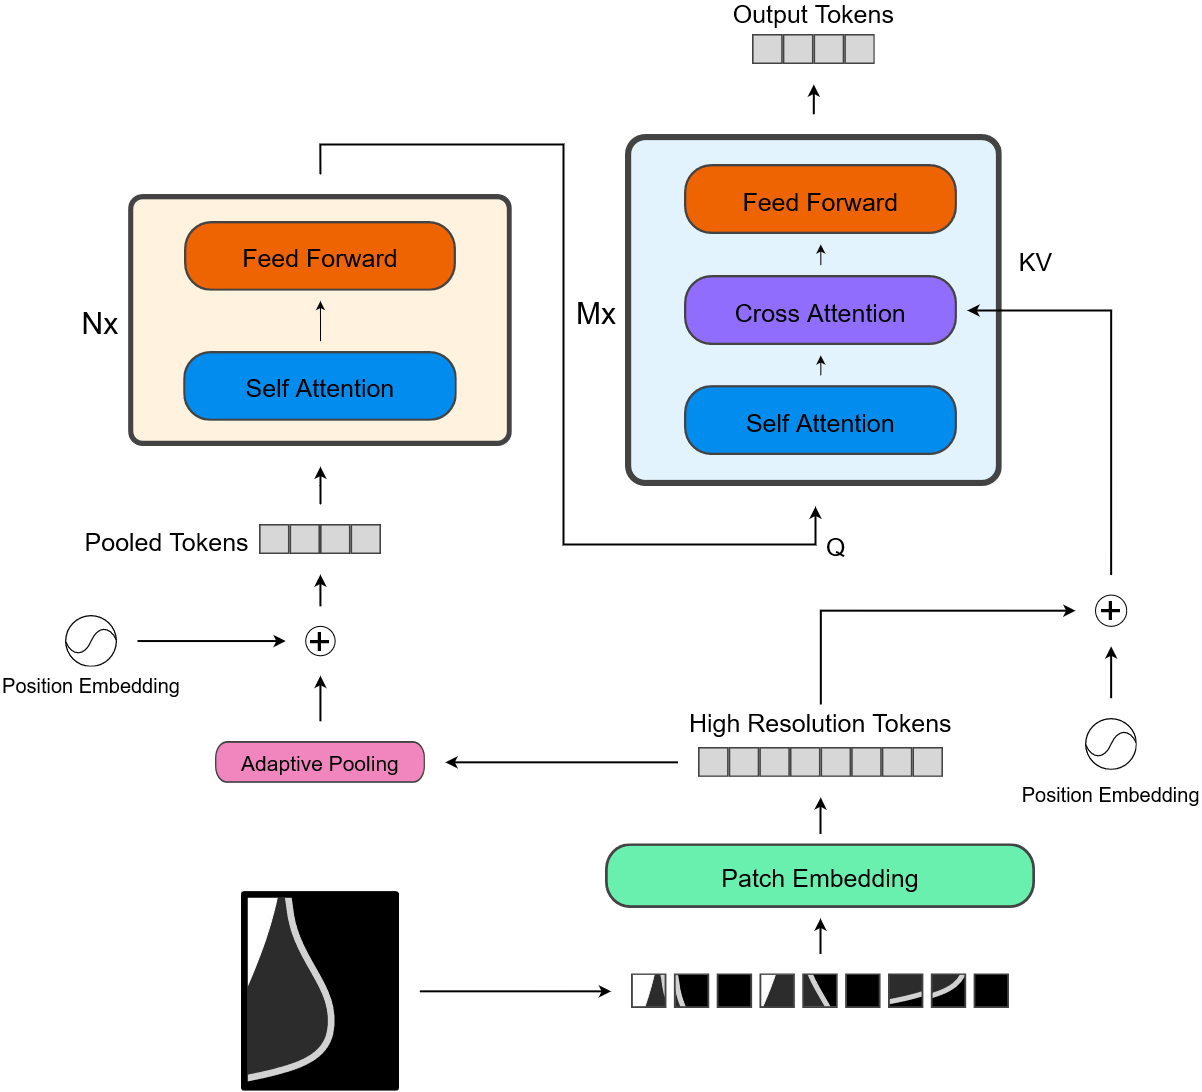
\includegraphics[width=0.75\textwidth]{./figures/avit.png}
    \caption{Adaptive Vision Transformer (AViT) Architecture}
    \label{fig:avit}
\end{figure}

A distinct feature of AViT is the placement of high resolution cross-attention layers at the end of the backbone. This is contrary to the typical design of isotropic backbones 
(which process at equal resolution throughout the backbone) and hierarchical backbones (which process at higher resolution towards the beginning of the backbone). This design choice
was made to enable the conversion of an existing ViT backbone into an AViT backbone, simply by adding layers to the end of the backbone. 
To further smooth the transition between ViT and AViT, we apply LayerScale \cite{touvron2021deeper} to all residual pathways of the additional AViT layers. In doing so, we set the initial condition of the transitioned AViT model to the output of the final ViT layer.
This easy conversion between standard and adaptive
models facilitates the scaling of existing backbones to higher resolutions with minimal retraining expense.


\subsection{Pre-training}

Self-supervised learning approaches have gained significant traction in recent years, particularly in the domain of medical imaging where labeled data is often scarce. 
In contrast to supervised learning, where a model is trained under the supervision of ground truth labels,
self-supervised learning methods learn useful representations from unlabeled data. 
While self-supervised learning offers advantages in leveraging unlabeled data and providing a strong foundation for various tasks, it's important to note its limitations. Self-supervised learning alone is typically insufficient to achieve optimal performance on a specific task and is usually followed by supervised fine-tuning on a smaller, labeled dataset.

Our research focused on developing a self-supervised learning method that could effectively handle the diverse nature of medical imaging data, including 1D, 2D, and 3D modalities.
Many existing contrastive and Siamese self-supervised methods, such as DINO \cite{caron2021emerging}, rely heavily on augmentations which may not translate well across all medical image domains. On the other hand, pixel-based methods like Masked Autoencoders (MAE) \cite{he2022masked}, while not making assumptions about the input data, may struggle with the inherent random variations present in medical data when tasked with pixel-level predictions.

To address these challenges, we adopted a Joint-Embedding Predictive Architecture (JEPA) \cite{assran2023self}. 
Figure \ref{fig:jepa} shows the application of JEPA to mammograms.
JEPA consists of three models: a student encoder, a teacher encoder with weights that trail the student encoder via exponential moving average, and a missing feature predictor.
For each partial image sent through the student encoder, a set of partial features is generated.
The missing feature predictor uses these partial features to predict values for some of the
features that are missing.
The predicted features are then compared against reference features generated by the application of the teacher encoder to the full image.

The JEPA approach offers several advantages for medical imaging applications, including:
\begin{enumerate}
    \item Generalizability: JEPA can be applied to various data dimensionalities (1D, 2D, 3D) without significant modifications.
      Any data that can be tokenized can be used with JEPA.
    \item Robustness: By focusing on predicting missing features rather than exact pixel values, JEPA is better equipped to handle the natural variations in medical data.
    \item Flexibility: The architecture allows for easy adaptation to different medical imaging modalities without relying on domain-specific augmentations.
\end{enumerate}

\begin{figure}
  \centering
  \includesvg[width=0.8\columnwidth]{figures/jepa.svg}
  \caption{A joint-embedding predictive architecture (JEPA) for mammograms \cite{assran2023self}.}
  \label{fig:jepa}
\end{figure}


We propose several modifications to the JEPA architecture to improve the model's performance and convergence rate, designating this modified architecture for medical imaging as M-JEPA.

\subsubsection{Loss Function}

Several adjustments are made to the typical JEPA loss function to improve the model's performance and convergence rate. 
A contrastive loss function is incorporated to encourage unique feature representations and mitigate mode collapse.
For minibatch feature predictions $F_i$ and $F_j$, the loss is computed as

\begin{equation}
  \mathcal{L}_c = \sum_{i \neq j} \max\Big(0, \cos\left(\bar{F}_i, \bar{F}_j\right) - \lambda\Big)
\end{equation}

where $\bar{F}_i$ and $\bar{F}_j$ are the average feature predictions for minibatch elements $i$ and $j$, respectively, 
and $\lambda$ is a margin controlling the desired dissimilarity between feature vectors. A $\lambda$ of $0.5$ is used for all experiments in this paper.

The typical JEPA loss function of mean squared error is replaced with a cosine similarity loss, which is found to yield superior performance when paired
with certain architectures. Another advantage of a cosine similarity loss is that it is independent of feature magnitude, reducing spikes in training
loss that would otherwise occur as feature magnitude changes.




\section{Data Analysis}
\noindent
% Describe how you analyzed your dataset and how you used the AIM-AHEAD Service Workbench cloud infrastructure and any other infrastructure used. (500-1000 words)

\subsection{CIFAR-10}

Experimentation using CIFAR-10 was done locally using a personal server with 3 RTX 3090 GPUs. The public availability and small size of CIFAR-10 make working
with this dataset extremely convenient. Ablation runs were conducted in parallel on each of the GPUs to accelerate the pace of iteration. Each RTX 3090 has 24GB of
video memory, enabling high batch sizes of $> 512$ with ease. 


\subsection{Mammographic Pre-training}

Training using the MedCognetics proprietary dataset was done on MedCognetics hardware due to restrictions on data access. MedCognetics training infrastructure
used consisted of 2 RTX 3090 GPUs, 24 CPU cores, and 128GB of RAM. Depending on the training configuration, RAM and CPU resources. Pre-processing of DICOM files
into 16-bit grayscale TIFFs was done using \href{https://github.com/medcognetics/torch-dicom}{torch-dicom}, an open source library provided by MedCognetics.
During preprocessing, any empty space is cropped away from the image before resizing to a fixed resolution. Resize operations are performed such that the aspect
ratio of the original image is preserved, with padding added when necessary to achieve the desired resolution. Tomosynthesis mammograms, which contain volumetric
data, are compressed into a 2D image by maximum intensity projection. DICOM metadata is organized into a SQL database

\subsection{EMBED}

Evaluation of MiT-UB using the EMBED dataset was conducted using the AIM-AHEAD Service Workbench cloud infrastructure. 
Models trained on the MedCognetics dataset were uploaded to Service Workbench, where the test set mammograms were processed
by the algorithms. The service workbench environment used an NVIDIA T4 GPU with 16GB of video memory, on which a throughput of 1-2 images/second was achieved.


\section{Research Findings and Results}
\noindent
% Describe the findings and results from the research project. What are the key insights and highlights of your research project? (1000-1200 words)

\subsection{CIFAR-10 Ablations}

Initial experimentation using CIFAR-10 focused on optimizing the JEPA architecture using linear probing accuracy as the evaluation metric.
Given the low resolution of CIFAR-10, the AViT variant of MiT-UB is not considered at this time.
The baseline JEPA architecture yielded a modest accuracy of $49.85\%$, but was found to be unstable and prone to mode collapse. Since
the JEPA architecture involves a student model attempting to predict features from a teacher model, mode collapse occurs when both the 
student and teacher learn to predict identical features for all inputs (e.g. all zeros). This solution space is undesirable and was addressed
through the incorporation of a contrastive loss term into the model's training procedure which improved stability and resulted in a higher 
accuracy of $66.28\%$. 

\begin{table}[H]
    \centering
    \begin{tabular}{p{0.67\linewidth}r}
        \toprule
        Model & Accuracy (\%) \\
        \midrule
        Supervised Baseline & 74.44 \\
        \midrule
        JEPA Baseline & 49.85$^{\dagger}$ \\
        +Contrastive Loss & 66.28$^{\dagger}$ \\
        +Cosine JEPA Loss & 63.76$^{\dagger}$ \\
        +SigSiLU & 70.15$^{\dagger}$ \\
        +Supervised Fine-Tuning & \textbf{81.97} \\
        \bottomrule
    \end{tabular}
    \caption{CIFAR-10 Validation Accuracies. Each row with a '+' indicates a cumulative change applied to the configuration of the previous row, building upon the JEPA Baseline. $^\dagger$Indicates results obtained through linear probing.}
    \label{tab:cifar10-accuracies}
\end{table}

After optimizing hyperparameters and increasing model size, a second round of ablations was conducted to determine the best activation function for the MLP layers of the ViT backbone.
At this point we adopt the fixed hyperparameters shown in Table \ref{tab:cifar10-hparams} for remaining CIFAR-10 ablations. 
A minimal set of augmentations is adopted for these ablations: random horizontal / vertical flipping and color jitter. The results of this ablation study are shown 
in Table \ref{tab:cifar10-accuracies-activation}. Given its strong performance, high sparsity, and computational efficiency, \reluTwo is selected as the default activation function in MiT-UB.

\begin{table}[H]
    \centering
    \begin{tabular}{p{0.4\linewidth}r}
        \toprule
        Hyperparameter & Value \\
        \midrule
        Optimizer & AdamW \\
        Learning Rate Schedule & One cycle cosine annealing \\
        Initial LR & \(0.0001\) \\
        Final LR & \(2 \times 10^{-6}\) \\
        Warmup Steps & \(5000\) \\
        Total Steps & \(50000\) \\
        Weight Decay & \(0.05\) \\
        \midrule
        Batch Size & \(512\) \\
        Precision & bf16-mixed \\
        \midrule
        Patch Size & \(4\) \\
        Model Dimension & \(384\) \\
        Head Dimension & \(32\) \\
        Depth & \(12\) \\
        Dropout & \(0.1\) \\
        \bottomrule
    \end{tabular}
    \caption{Hyperparameters adopted for subsequent CIFAR-10 ablations.}
    \label{tab:cifar10-hparams}
\end{table}


\begin{table}[H]
    \centering
    \begin{tabular}{p{0.15\linewidth}p{0.4\linewidth}r}
        \toprule
        Activation & Formulation & Accuracy (\%) \\
        \midrule
        GELU & \( x \cdot \frac{1}{2} \left[1 + \mathrm{erf}\left(\frac{x}{\sqrt{2}}\right)\right] \) & 78.02$^{\dagger}$ \\
        SiLU & \( x \cdot \sigma(x) \) & 74.92$^{\dagger}$ \\
        ReLU & \( \max(0, x) \) & 76.60$^{\dagger}$ \\
        \reluTwo & \( \max(0, x)^2 \) & \textbf{79.29}$^{\dagger}$ \\
        \midrule
        GLU & \( (\mathbf{W}_1 \mathbf{x} + \mathbf{b}_1) \odot \sigma(\mathbf{W}_2 \mathbf{x} + \mathbf{b}_2) \) & X \\
        SwiGLU & \( \mathrm{SiLU}(\mathbf{W}_1 \mathbf{x} + \mathbf{b}_1) \odot (\mathbf{W}_2 \mathbf{x} + \mathbf{b}_2) \) & 77.58$^{\dagger}$ \\
        SigSiLU & \( \mathrm{SiLU}(\mathbf{W}_1 \mathbf{x} + \mathbf{b}_1) \odot \sigma(\mathbf{W}_2 \mathbf{x} + \mathbf{b}_2) \) & 79.18$^{\dagger}$ \\
        \bottomrule
    \end{tabular}
    \caption{Ablation results of MLP activation functions in MiT-UB. $^\dagger$Indicates results obtained through linear probing. GLU failed to converge.}
    \label{tab:cifar10-accuracies-activation}
\end{table}


Next, we explore methods of improving the performance of MiT-UB on CIFAR-10 using fine tuning strategies. Three fine tuning methods are considered:

\begin{enumerate}
    \item End to end supervised fine tuning at a lower learning rate.
    \item Low-Rank Adaptation (LoRA) \cite{hu2021lora} fine tuning on attention and MLP layers, with unfrozen patch embedding and LayerNorm layers.
    \item Removing the stop-gradient operation from the M-JEPA linear probe.
\end{enumerate}

Performance of these methods is compared in Table \ref{tab:cifar10-tune-method}. For LoRA fine tuning a rank and scale factor of $32$ are adopted. A fresh supervised baseline is established using the optimized design found from previous
ablations and hyperparameter optimization.

\begin{table}[H]
    \centering
    \begin{tabular}{p{0.4\linewidth}r}
        \toprule
        Method & Accuracy (\%) \\
        \midrule
        Fully Supervised & 80.3 \\
        \midrule
        Supervised Fine-Tuning & \textbf{87.5} \\
        LoRA Fine-Tuning &  83.7 \\
        M-JEPA Without Stop-Gradient & 85.1 \\
        \bottomrule
    \end{tabular}
    \caption{Comparison of fine tuning methods on CIFAR-10.}
    \label{tab:cifar10-tune-method}
\end{table}

Supervised fine tuning at a lower learning rate is found to be the most effective method of fine tuning MiT-UB on CIFAR-10. However LoRA does present advantages
in terms of parameter efficiency and lower train-test performance disparity when compared to standard fine tuning. At $87.5\%$ accuracy, MiT-UB is approaching the
performance of a ConvNeXT \cite{liu2022convnext} baseline which achieves $91.6\%$ accuracy purely from supervised training.

\subsection{Mammography}

The optimized backbone design found through CIFAR-10 ablations is scaled up for application to mammograms. A model dimension of $768$ and depth of $24$
is selected, yielding a backbone of $155\mathrm{M}$ parameters. A head dimension of $64$ is selected, the maximum allowed under Flash Attention \cite{dao2022flash}
on a RTX 3090 GPU. Training is conducted in three stages, starting with low resolution ViT training, followed by high resolution AViT training, and finally
supervised fine tuning of the AViT backbone on breast cancer triage. These stages are summarized in Table \ref{tab:mammo-training}.
Table \ref{tab:mammo-val-metrics} reports the primary metric and value for each training stage. Breast cancer triage AUROC
for validation data is computed on a per-study basis by computing the maximum of individual image scores within a study.

\begin{table}[H]
    \centering
    \begin{tabular}{l r r r r r}
        \toprule
        Training Stage & Backbone & Resolution & Steps & Batch Size &Wall Time \\
        \midrule
        M-JEPA Phase 1 & ViT & \(512\times384\) & \(250000\) & \(64\) & \(56\) hours \\
        M-JEPA Phase 2 & AViT & \(3072\times2304\) & \(150000\) & \(16\) & \(51\) hours \\
        Supervised Fine-Tuning & AViT & \(3072\times2304\) & \(500000\) & \(8\) & \(97\) hours \\
        \bottomrule
    \end{tabular}
    \caption{Training stages for MiT-UB on mammograms.}
    \label{tab:mammo-training}
\end{table}



\begin{table}[H]
    \centering
    \begin{tabular}{l r r}
        \toprule
        Training Stage & Metric & Value \\
        \midrule
        M-JEPA Phase 1 & View Classification Accuracy & \(99.9\dagger\) \\
        M-JEPA Phase 2 & View Classification Accuracy & \(99.49\dagger\) \\
        Supervised Fine-Tuning & Breast Cancer Triage AUROC & \(0.8603\) \\
        \bottomrule
    \end{tabular}
    \caption{Primary validation metric and result for each training stage. $^\dagger$Indicates results obtained through linear probing.}
    \label{tab:mammo-val-metrics}
\end{table}

This model was then tested on breast cancer triage performance on the EMBED test set. Each of the four standard views was independently processed to compute a triage score. Triage scores within breasts were averaged, and scores between breasts were reduced using a maximum operation. This yields a single triage score for each exam on which performance is evaluated.
A visualization of case score computation is shown in Figure \ref{fig:case-score}.
AUROC is considered the primary evaluation metric, but thresholded metrics like sensitivity and specificity are also reported using a fixed threshold of $0.5$, the results of which are shown in Table \ref{tab:triage-cohort}. The model achieves a performance in line with its validation performance, indicating that the model is well calibrated for the task of mammographic breast cancer triage.
For brevity this report focuses stratified analysis on the patient's race, the results of which are shown in Table \ref{tab:triage-race}. In cohorts with sufficient sample size the algorithm achieves comparable performance across racial groups. Unforunately the limited number of malignant exams for racial groups other than white and African-American limit the ability to draw conclusions about the model's performance across these groups.


\begin{figure}[H]
    \centering
    \includesvg[width=0.85\textwidth]{./figures/case_score.svg}
    \caption{Case score reduction. Scores for each breast are averaged, and scores between breasts are reduced by a maximum.}
    \label{fig:case-score}
\end{figure}

\begin{table}[H]
    \centering
    \begin{tabular}{lr}
\toprule
 & Triage Performance \\
\midrule
Samples & 1052 \\
Positive & 526 \\
Negative & 526 \\
AUC & 0.8494 \\
AUC\textsubscript{LB} & 0.8244 \\
AUC\textsubscript{UB} & 0.8744 \\
TP & 492 \\
FP & 184 \\
TN & 342 \\
FN & 34 \\
NPV & 0.9096 \\
PPV & 0.7278 \\
Accuracy & 0.7928 \\
Sensitivity & 0.9354 \\
Sensitivity\textsubscript{LB} & 0.9183 \\
Sensitivity\textsubscript{UB} & 0.9544 \\
Specificity & 0.6502 \\
Specificity\textsubscript{LB} & 0.6160 \\
Specificity\textsubscript{UB} & 0.6863 \\
\bottomrule
\end{tabular}

    \caption{Triage performance metrics for the MiT-UB (AViT) model on the cohort dataset.}
    \label{tab:triage-cohort}
\end{table}


\begin{table}[H]
    \centering
    \resizebox{\textwidth}{!}{%
        \begin{tabular}{lrrrrrrrr}
\toprule
Race & Black & American Indian & Asian & White & Hispanic & Multiple & Pacific Islander & Unknown \\
\midrule
Samples & 426 & 529 & 57 & 394 & 50 & 4 & 3 & 115 \\
Positive & 234 & 526 & 27 & 235 & 19 & 2 & 1 & 8 \\
Negative & 192 & 3 & 30 & 159 & 31 & 2 & 2 & 107 \\
AUC & 0.8178 & 0.7243 & 0.8889 & 0.8178 & 0.9117 & 1 & 1 & 0.9089 \\
AUC\textsubscript{LB} & 0.7715 & 0.4636 & 0.7827 & 0.7690 & 0.8164 & 1 & 1 & 0.8328 \\
AUC\textsubscript{UB} & 0.8605 & 0.9684 & 0.9654 & 0.8675 & 0.9846 & 1 & 1 & 0.9685 \\
TP & 217 & 492 & 25 & 221 & 18 & 2 & 1 & 8 \\
FP & 74 & 2 & 8 & 67 & 11 & 0 & 0 & 22 \\
TN & 118 & 1 & 22 & 92 & 20 & 2 & 2 & 85 \\
FN & 17 & 34 & 2 & 14 & 1 & 0 & 0 & 0 \\
NPV & 0.8741 & 0.0286 & 0.9167 & 0.8679 & 0.9524 & 1 & 1 & 1 \\
PPV & 0.7457 & 0.9960 & 0.7576 & 0.7674 & 0.6207 & 1 & 1 & 0.2667 \\
Accuracy & 0.7864 & 0.9319 & 0.8246 & 0.7944 & 0.7600 & 1 & 1 & 0.8087 \\
Sensitivity & 0.9274 & 0.9354 & 0.9259 & 0.9404 & 0.9474 & 1 & 1 & 1 \\
Sensitivity\textsubscript{LB} & 0.9017 & 0.9202 & 0.8519 & 0.9106 & 0.8421 & 1 & 1 & 1 \\
Sensitivity\textsubscript{UB} & 0.9530 & 0.9544 & 1 & 0.9617 & 1 & 1 & 1 & 1 \\
Specificity & 0.6146 & 0.3333 & 0.7333 & 0.5786 & 0.6452 & 1 & 1 & 0.7944 \\
Specificity\textsubscript{LB} & 0.5573 & 0 & 0.5667 & 0.5157 & 0.5161 & 1 & 1 & 0.7290 \\
Specificity\textsubscript{UB} & 0.6719 & 0.6667 & 0.8667 & 0.6478 & 0.7742 & 1 & 1 & 0.8598 \\
\bottomrule
\end{tabular}

    }
    \caption{Triage performance metrics for the MiT-UB (AViT) model by race.}
    \label{tab:triage-race}
\end{table}


\section{Lessons Learned}
\noindent
% Describe the success and challenges that arise from the research project. (250-500 words)

A significant lesson learned during the course of this project is the pitfall of premature optimization. Many methods with a strong
theoretical motivation were proposed and implemented through highly optimized GPU kernels, only for the method to fail to deliver
any performance benefit over existing baselines. Large amounts of time and effort were spent prematurely optimizing these methods,
a waste of resources that could have been mitigated by more thoroughly testing unoptimized versions of the proposed methods.

Conversely, a major success of this project was in how the characteristics of the vision transformer were leveraged to a positive end. Much attention is paid to the quadratic complexity of the self attention operation in ViTs and their ineffectiveness in data constrained environments. However, ViT's strengths of permutation invariance, cardinality invariance, and receptive field deformability are strengths that can be exploited to a useful end. In particular, the paradigm of adding adaptive layers to a ViT backbone to form an AViT architecture is a clever way to scale ViTs from existing backbones.

Finally, a lesson for future fellows working with the EMBED dataset (specifically the subset available to research fellows) is to be mindful of its relatively limited population of malignant exams. Based on the prevalence of cancer in the U.S. screening population, an enriched test set of $N \geq 400$ malignant studies is desirable. Creating a test set of this size would leave less than $300$ patients with malignant findings for training and validation of a model. Fellow may wish to consider supplementing the EMBED dataset with additional mammograms from public datasets, or pursuing research questions that leverage EMBED's large population of benign studies.

\section{Conclusion}
\noindent
% Restate your research topic, restate your research question, summarize and connect the results of the findings, and conclude your final thoughts. (250-500 words)

This research project proposed and evaluated a new vision transformer architecture for medical imaging with a focus on
self supervised learning techniques in order to improve algorithmic performance on minority cohorts and mitigate the impact in label bias.
A Joint-Embedding Predictive Architecture was chosen as the foundation for self supervised learning and augmented with a series of modifications to improve performance and stability, which we term M-JEPA. Ablations using M-JEPA were conducted on CIFAR-10 to optimize the design of MiT-UB in a limited training data environment. From these ablations we observed a maximum linear probing accuracy of $79.29\%$ and a maximum supervised fine-tuning accuracy of $87.5\%$. The accuracy achieved by linear probing rivals the accuracy obtained by supervised training from scratch ($80.3\%$) and the fine-tuning accuracy approaches the performance of a supervised ConvNeXT baseline ($91.6\%$). These results indicate that M-JEPA can effectively leverage a limited pool of unlabeled data to learn feature representations that are useful for downstream tasks.
Additionally, the significant increase in accuracy between supervised training from scratch and fine-tuning with M-JEPA pre-training suggests that M-JEPA pre-training can improve performance in conditions where labeled data is limited or expensive to obtain.

Using the optimizations discovered through CIFAR-10, we apply MiT-UB to the task of mammographic breast cancer triage. 
A $150\mathrm{M}$ parameter MiT-UB backbone was selected for this task, and training was conducted in three stages. First, a low resolution ViT backbone was trained on a large dataset of unlabeled mammograms. Next, the ViT backbone was converted into an AViT backbone and fine-tuned at a higher resolution on the same dataset. Finally, the AViT backbone was fine-tuned at high resolution on a smaller dataset of labeled mammograms with a focus on breast cancer triage performance.
When evaluated on the EMBED test set the model achieves a breast cancer triage AUROC of $0.8494$. Comparable performance is achieved on racial subroups for which there is a sufficient number of malignant exams for testing.

Future work could further optimize MiT-UB, explore self supervised training tasks beyond M-JEPA, conduct additional stratified analysis using EMBED, or curate supplemental testing data that represents a more diverse set of patients.


\pagebreak
\section{References}
\noindent
% Add all of the references you used for your research.
\renewcommand{\refname}{}
\bibliographystyle{plain}
\bibliography{references}

\vspace{4\baselineskip}
\noindent
\textbf{I hereby attest that my research project is complete.}

\vspace{1cm}
\noindent X \underline{\hspace{10cm}}  \\
\\
\noindent \textbf{Name Print:} Scott Chase Waggener \hfill \textbf{Date:} \today

\end{document}
